%%%%%%%%%%%%%%%%%%%%%%%%%%%%%%%%%%%%%%%%%
% Masters/Doctoral Thesis 
% LaTeX Template
% Version 2.5 (27/8/17)
%
% This template was downloaded from:
% http://www.LaTeXTemplates.com
%
% Version 2.x major modifications by:
% Vel (vel@latextemplates.com)
%
% This template is based on a template by:
% Steve Gunn (http://users.ecs.soton.ac.uk/srg/softwaretools/document/templates/)
% Sunil Patel (http://www.sunilpatel.co.uk/thesis-template/)
%
% Template license:
% CC BY-NC-SA 3.0 (http://creativecommons.org/licenses/by-nc-sa/3.0/)
%
%%%%%%%%%%%%%%%%%%%%%%%%%%%%%%%%%%%%%%%%%

%----------------------------------------------------------------------------------------
%	PACKAGES AND OTHER DOCUMENT CONFIGURATIONS
%----------------------------------------------------------------------------------------

\documentclass[
11pt, % The default document font size, options: 10pt, 11pt, 12pt
%oneside, % Two side (alternating margins) for binding by default, uncomment to switch to one side
british, % ngerman for German
singlespacing, % Single line spacing, alternatives: onehalfspacing or doublespacing
%draft, % Uncomment to enable draft mode (no pictures, no links, overfull hboxes indicated)
%nolistspacing, % If the document is onehalfspacing or doublespacing, uncomment this to set spacing in lists to single
%liststotoc, % Uncomment to add the list of figures/tables/etc to the table of contents
%toctotoc, % Uncomment to add the main table of contents to the table of contents
%parskip, % Uncomment to add space between paragraphs
%nohyperref, % Uncomment to not load the hyperref package
headsepline, % Uncomment to get a line under the header
%chapterinoneline, % Uncomment to place the chapter title next to the number on one line
%consistentlayout, % Uncomment to change the layout of the declaration, abstract and acknowledgements pages to match the default layout
]{MastersDoctoralThesis} % The class file specifying the document structure

\usepackage[utf8]{inputenc} % Required for inputting international characters
\usepackage[T1]{fontenc} % Output font encoding for international characters
\usepackage{abstract}
\usepackage{mathpazo} % Use the Palatino font by default
\usepackage[backend=bibtex,natbib=true]{biblatex} % Use the bibtex backend with the authoryear citation style (which resembles APA)
\def\changemargin#1#2{\list{}{\rightmargin#2\leftmargin#1}\item[]}
\let\endchangemargin=\endlist 
\addbibresource{biblio.bib} % The filename of the bibliography
%\renewcommand\acknowledgementsname{Remerciements}
\usepackage[autostyle=true]{csquotes} % Required to generate language-dependent quotes in the bibliography
\newcommand{\mc}[2]{\multicolumn{#1}{|c|}{#2}}
\usepackage{blindtext}
\usepackage{tabularx}
%----------------------------------------------------------------------------------------
%	MARGIN SETTINGS
%----------------------------------------------------------------------------------------

\geometry{
	paper=a4paper, % Change to letterpaper for US letter
	inner=2.5cm, % Inner margin
	outer=3.8cm, % Outer margin
	bindingoffset=.5cm, % Binding offset
	top=1.5cm, % Top margin
	bottom=1.5cm, % Bottom margin
	%showframe, % Uncomment to show how the type block is set on the page
}


\begin{document}

\frontmatter % Use roman page numbering style (i, ii, iii, iv...) for the pre-content pages

\pagestyle{plain} % Default to the plain heading style until the thesis style is called for the body content

%----------------------------------------------------------------------------------------
%	TITLE PAGE
%----------------------------------------------------------------------------------------

\begin{titlepage}
\begin{center}

\begin{figure}[h]
\centering
\includegraphics[width=14cm]{Images/logos.jpg}
\end{figure}

\vspace*{.06\textheight}
{\scshape\LARGE {Université catholique de Louvain}\par}\vspace{1.5cm} % University name
%\textsc{\Large Doctoral Thesis}\\[0.5cm] % Thesis type

\HRule \\[0.4cm] % Horizontal line
\begin{changemargin}{-0.5cm}{-0.5cm} 
{\huge \bfseries {Study of the stress relieve heat-treatment of}\\
 \vspace{0.2cm}\hspace{0.2cm} \huge \bfseries {additively manufactured AlSi10Mg alloy:}}\vspace{0.3cm}

\LARGE{Influence on microstructure and mechanical properties}\par
\end{changemargin} 
\HRule \\[1.5cm] % Horizontal line
 \vspace{1cm}
\large \textit{Dissertation presented by}\\
\vspace{0.5cm}
\begin{minipage}[t]{0.35\textwidth}
\begin{flushleft} \large
David DISPAS
\end{flushleft}
\end{minipage}
\large \textit{and}
\begin{minipage}[t]{0.35\textwidth}
\begin{flushright} \large
Arthur BOUILLOT
\end{flushright}
\end{minipage}\\%[3cm]
 
\vspace{0.6cm}
\large \textit{for obtaining the Master’s degree in}\\[0.3cm] 
\vspace{0.20cm}
\begin{minipage}[t]{0.41\textwidth}
\begin{flushleft} \large
Mechanical Engineering
\end{flushleft}
\end{minipage}
\large \textit{and}
\begin{minipage}[t]{0.4\textwidth}
\begin{flushright} \large
Chemical and Materials \\
\centering \hspace{0.7cm} Engineering
\end{flushright}
\end{minipage}\\%[1cm]
\vspace{0.7cm}
\large \textit{at Ecole Polytchnique de Louvain (EPL)}\\[1.3cm]
\vfill
\large {\textit{Supervisor:} Aude SIMAR}
%\textit{in the}\\[0.4cm]
\vfill
%\groupname\\\deptname\\[2cm] % Research group name and department name
 \large {\textit{Readers:} Laurent DELANNAY, Anne MERTENS, Camille VAN DER REST}
%\vfill
\vfill
{\large Academic year 2017-2018}\\%[1cm] % Date
%\includegraphics{Logo} % University/department logo - uncomment to place it
 

\end{center}
\end{titlepage}

%---------------------------------------------------------------------
%%	QUOTATION PAGE
%%----------------------------------------------------------------------------------------

\vspace*{0.2\textheight}

\noindent\enquote{\itshape Citation stylée.}\bigbreak

\hfill Mec cool

%----------------------------------------------------------------------------------------
%	ABSTRACT PAGE
%----------------------------------------------------------------------------------------

%\begin{abstract}
%%\addchaptertocentry{Résumé} % Add the abstract to the table of contents
%The Thesis Abstract is written here (and usually kept to just this page). The page is kept centered vertically so can expand into the blank space above the title too\ldots
%\end{abstract}

%----------------------------------------------------------------------------------------
%	ACKNOWLEDGEMENTS
%----------------------------------------------------------------------------------------

\chapter*{Acknowledgements}

%\addchaptertocentry{Remerciements} % Add the acknowledgements to the table of contents
Blablabla. blabla. bla.
%\end{acknowledgements}

%----------------------------------------------------------------------------------------
%	LIST OF CONTENTS/FIGURES/TABLES PAGES
%----------------------------------------------------------------------------------------

\tableofcontents % Prints the main table of contents

\listoffigures % Prints the list of figures

\listoftables % Prints the list of tables

%----------------------------------------------------------------------------------------
%	ABBREVIATIONS
%----------------------------------------------------------------------------------------

\begin{abbreviations}{ll} % Include a list of abbreviations (a table of two columns)
%
\textbf{AM} & \textbf{A}dditive \textbf{M}anufacturing\\
\textbf{CAD} & \textbf{C}omputer \textbf{A}ided \textbf{D}esign\\
\textbf{DMLS} & \textbf{D}irect \textbf{M}etal \textbf{L}aser \textbf{S}intering\\
\textbf{DMP} & \textbf{D}irect \textbf{M}etal \textbf{P}rinter\\
\textbf{ICP} & \textbf{I}nductively \textbf{C}oupled \textbf{P}lasma\\
\textbf{SEM} & \textbf{S}canning \textbf{E}lectron \textbf{M}icroscope\\
\textbf{SLM} & \textbf{S}elective \textbf{L}aser \textbf{M}elting\\

%\textbf{WSF} & \textbf{W}hat (it) \textbf{S}tands \textbf{F}or\\
%
\end{abbreviations}

%----------------------------------------------------------------------------------------
%	PHYSICAL CONSTANTS/OTHER DEFINITIONS
%----------------------------------------------------------------------------------------
%
%\begin{constants}{lr@{${}={}$}l} % The list of physical constants is a three column table
%
%% The \SI{}{} command is provided by the siunitx package, see its documentation for instructions on how to use it
%
%Speed of Light & $c_{0}$ & \SI{2.99792458e8}{\meter\per\second} (exact)\\
%%Constant Name & $Symbol$ & $Constant Value$ with units\\
%
%\end{constants}

%----------------------------------------------------------------------------------------
%	SYMBOLS
%----------------------------------------------------------------------------------------

\chapter*{Symbols}%{lll} % Include a list of Symbols (a three column table)
\begin{tabular}{lll}

\centering

$D_a$ & Average particle size & $[\mu m]$\\ 
$E_d$ & Volumetric energy density & $[\frac{J}{mm^3}]$\\
$h$ & Hatch space & $[\mu m]$\\
$H_v$ & Vickers hardness & $[HV]$\\
$P$ & Laser power & $[W]$ \\
$p_{O_2}$ & Oxygen pressure & $[mbar]$\\
$t$ & Layer thickness & $[\mu m]$\\
$v_s$ & Scanning speed & $[\frac{mm}{s}]$ \\
$W_a$ & Specimen dry weight& $ [g]$ \\
$W_w$ & Specimen underwater weight & $[g]$\\
\addlinespace
\addlinespace
$\phi_{99\%}$ & Laser spot size at the 99\% contour & $[\mu m]$\\
$\lambda$ & Laser wavelength & $[nm]$\\
$\rho_{a}$ & Apparent density & $[\frac{g}{cm^3}$] \\
$\rho_{w}$ & Water density & $[\frac{g}{cm^3}$]\\
$\rho_{rel}$ & Apparent relative density & $[-]$ \\

%\addlinespace % Gap to separate the Roman symbols from the Greek

%$\omega$ & angular frequency & \si{\radian} \\
\end{tabular}
%\end{symbols}

%----------------------------------------------------------------------------------------
%	DEDICATION
%----------------------------------------------------------------------------------------

\dedicatory{Nous dédions ce travail à nos familles et amis} 

%----------------------------------------------------------------------------------------
%	THESIS CONTENT - CHAPTERS
%----------------------------------------------------------------------------------------

\mainmatter % Begin numeric (1,2,3...) page numbering

\pagestyle{thesis} % Return the page headers back to the "thesis" style

% Include the chapters of the thesis as separate files from the Chapters folder
% Uncomment the lines as you write the chapters

\chapter{Introduction}
\label{Chap1}

This is, with the concluding chapter, a significant portion of memory. This should
especially present the context and objectives of the work. Generally, the memory structure (content
of chapters) is briefly exposed

\chapter{Etat de l'art}
\label{Chap2}
Les caractérisitiques des pièces produites grâce à la fusion laser sélective (SLM) sont le fruit de l'action simultanée et couplée d'un grand nombres de paramètres (voir figure \ref{fig:param} ) \parencite{Aboulkair140820}. Les résultats sont très sensibles à leurs variations et il est donc nécessaire de les contrôler méticuleusement. Pour ces raisons, il n'est pas simple d'étudier leurs impacts.\\

Durant les dernières années, les travaux visant à optimiser les conditions de fabrication se sont multipliés. La minimisation de la porosité est au centre de l'attention: elle est en effet liée à la qualité des propriétés mécaniques. De plus au delà d'un seuil, des risques de rupture prématurée peuvent apparaitre (source). (Initiation de sites de propag ... ) On s'intéresse ensuite à optimiser d'autres caractéristiques du matériau et à la productivité de la technique.


\begin{figure}[th]
\centering
\includegraphics[scale=0.42]{Images/Param}
\decoRule

\caption[Paramètres entrant en jeu dans le procédé LSM]{Paramètres entrant en jeu dans le procédé LSM}
\label{fig:param}
\end{figure}

%Recherches biblio....
%\section{Comment référencer?}
%The \code{biblatex} package is used to format the bibliography and inserts references such as this one \parencite{Reference1}. The options used in the \file{main.tex} file mean that the in-text citations of references are formatted with the author(s) listed with the date of the publication. Multiple references are separated by semicolons (e.g. \parencite{Reference2, Reference1}) and references with more than three authors only show the first author with \emph{et al.} indicating there are more authors (e.g. \parencite{Reference3}). This is done automatically for you. %To see how you use references, have a look at the \file{Chapter1.tex} source file. Many reference managers allow you to simply drag the reference into the document as you type.
%
%Scientific references should come \emph{before} the punctuation mark if there is one (such as a comma or period). The same goes for footnotes\footnote{Such as this footnote, here down at the bottom of the page.}. You can change this but the most important thing is to keep the convention consistent throughout the thesis. Footnotes themselves should be full, descriptive sentences (beginning with a capital letter and ending with a full stop). The APA6 states: \enquote{Footnote numbers should be superscripted, [...], following any punctuation mark except a dash.} The Chicago manual of style states: \enquote{A note number should be placed at the end of a sentence or clause. The number follows any punctuation mark except the dash, which it precedes. It follows a closing parenthesis.}
%
%The bibliography is typeset with references listed in alphabetical order by the first author's last name. This is similar to the APA referencing style. To see how \LaTeX{} typesets the bibliography, have a look at the very end of this document (or just click on the reference number links in in-text citations).

\chapter{Materials and methods}
\label{Chap3}
\section{Powder follow-up}

\subsection{Sieving}

\subsection{Grain size and distribution}

\subsection{Composition}

%\subsection{Drying}

\section{SLM manufacturing}
\label{MMFPP}
The same direct metal printer (DMP) was used to fabricate all specimens throughout this work. It is a \textit{ProX DMP 200} printer, manufactured by \textit{3D Systems} (see figure \ref{fig:Printer}). It uses a laser with a theoretical maximal power of 300 [W] and wavelength $\lambda$ = 1070 [nm] \parencite{3D}. Its actual maximal power is $P_{max}=273.6 [W]$. \textcolor{gray}{[QUEL EST LE SPOT SIZE?]}  The maximal envelope capacity of the machine (W x D x H) is 140 x 140 x 125 [mm]. Its typical accuracy is +/- 50 [$\mu m$] for small parts and +/- 0.2\% for large parts. It allows for the set-up of a protection atmosphere. However, it does not integrate any heating feature for the build bed.\\

\begin{figure}[ht]
\centering
\includegraphics[scale=0.7]{Images/Printer}
\decoRule
\caption[ProX DMP 200 printer]{ProX DMP 200 printer (from the user's ProX DMP 200 general instructions document).}
\label{fig:Printer}
\end{figure}

In this thesis, argon was used as shielding gas. The composition of the gas environment was monitored so as to keep $p_{O2}$ < 500 [ppm]. Laser compensations were set to take into account the excess energy at the start and end of the scanning vectors (see figure \ref{fig:Compens}). These were chosen in accordance with the manufacturer recommendations (figure \ref{fig:Compens1}). Values for hatch space (h) and layer thickness (t) were respectively set to 100 [$\mu m$] and 30 [$\mu m$]. The scan speed ($v_s$) and the laser power (P) were varied in the ranges [900 ; 1500] [$\frac{mm}{s}$] and [$0.75 \cdot P_{max}$ ; $P_{max}$] respectively, in order to optimise of the built specimens (see section \ref{Rparaopti}). Educated guesses were made based on literature and previous works done at the UCL. The parameters used are resumed in appendix \ref{ppa}. Batches were named in the format X200-\textit{yymmdd}. The prefix "X200" refers to the DMP used. It is followed by the date of printing (6 digits). Recycled powder was used for every batch except for X200-180222 and X200-180228. Figures with detailed specimens positions, denominations, scanning orders and sintering durations for all batches are available in appendix \ref{mda}.\\

\begin{figure}[ht]
\centering
\includegraphics[scale=0.3]{Images/Compens}
\decoRule
\caption[Melt pool contours with and without laser compensation (exaggeration)]{Melt pool contours with and without laser compensation (exaggeration).}
\label{fig:Compens}
\end{figure}

\begin{figure}[ht]
\centering
\includegraphics[scale=0.45]{Images/Compens1}
\decoRule
\caption[Laser compensations as a function of the scanning speed (as recommended by the manufacturer)]{Laser compensations as a function of the scanning speed (as recommended by the manufacturer).}
\label{fig:Compens1}
\end{figure}

The batches were first prepared on \textit{DMP ProX Manufacturing}, a dedicated CAD software. It enabled to select the values for the parameters previously mentioned, as well as the position of the specimens. For this thesis, all cylinders and tensile specimens were fabricated vertically. The dimensions notations for the samples types and the tensile specimens detailed geometry are gathered on figure \ref{fig:cc}. 

\begin{figure}[ht]
\centering
\noindent\makebox[\textwidth]{\includegraphics[scale=0.52]{Images/cc}}
\decoRule
\caption[Dimensions notations for (a) cubic specimens (b) cylindrical specimens (c) parallelepiped specimens (d) tensile specimen]{Dimensions notations for (a) cubic specimens (b) cylindrical specimens (c) parallelepiped specimens (d) tensile specimens with dimensions in [mm]}
\label{fig:cc}
\end{figure}


An island scanning strategy was chosen on account of research done on the subject (see section \ref{pp}). It is a hexagonal pattern. The replicated hexagon's smallest width is equal to 5 [mm]. An overlap of 100 [$\mu m$] was set, as illustrated on figure \ref{fig:OL}. There is a rotation of $90^\circ$ and a translation of a third of basis vector between two successive powder layers as depicted by figure \ref{fig:Lassup}. In the case of a contour scanning strategy, the contours were pre scanned for each powder layer with the same P and $v_s$ used for the bulk (see figure \ref{fig:LasCSC}). The scanning order among the samples was automatically chosen. \\

\begin{figure}[ht]
\centering
\includegraphics[scale=0.27]{Images/OL}
\decoRule
\caption[Schematic representation of the hexagonal pattern scanning strategy]{Schematic representation of the hexagonal pattern scanning strategy}
\label{fig:OL}
\end{figure}

\begin{figure}[ht]
\centering
\noindent\makebox[\textwidth]{\includegraphics[scale=0.3]{Images/Lassup}}
\decoRule
\caption[Screen capture of the laser scanning pattern for a parallelepiped sample: (a) Layer $n$ (b) Layer $n+1$ (c) Layer $n+2$]{Laser scanning pattern for a parallelepiped sample: (a) Layer $n$ (b) Layer $n+1$ (c) Layer $n+2$}
\label{fig:Lassup}
\end{figure}

\begin{figure}[ht]
\centering
\noindent\makebox[\textwidth]{\includegraphics[scale=0.4]{Images/LasCSC}}
\decoRule
\caption[Screen capture of the laser path for a cylindric sample (a) with contour scanning strategy (b) without contour scanning strategy]{Screen capture of the laser path for a cylindric sample (a) with contour scanning strategy (b) without contour scanning strategy}
\label{fig:LasCSC}
\end{figure}
\section{Heat treatments}
\label{MMHT}
The heat treatments were conducted inside a unique oven of the VT 5050 EKP model, manufactured by Heraeus, which is able to reach a temperature of 400$^\circ$ C. Samples temperature data was obtained through a thermocouple welded to the sample surface, thanks to a ... . \textcolor{gray}{[Méthode de soudage, élévation de la température durant l'opération]} The data was displayed and saved every 10 seconds, with a precision of 0.1$^\circ$ C, thanks to a Agilent 34972A LXI Data Acquisition/Switching Unit, connected to the thermocouple (see Fig. for both devices). For unknown reasons, that can not be explained only by thermal inertia, setting the oven to the target temperature proved unable to heat the specimens to the same temperature. After a couple samples for testing, the method applied for following ones was to set the oven at a temperature about 20$^\circ$ C above the target, so that the data acquisition unit connected to the thermocouple displays the right temperature.\\

Due to the inaccuracy of the oven, maintaining the samples at the exact target temperature has not proved possible. The holding plateaus were thus rather slow increasing slopes. For most of the samples, the theoretical beginning of the holding was set when the specimen reached a temperature 5$^\circ$ C below the target value, so that the sample average temperature for the complete holding was the closest possible to target value.\\

Samples that were subject to a heat treatment were named in a particular format, to ease distinction between them. They received the name of the batch, followed by "TT-\textit{holdingtemperature-holdingtime-specificities}". Cubes that were subject to heat treatments were 5 x 5 x 5 [mm$^3$].\\

%\begin{figure}[ht]
%	\centering
%	\includegraphics[scale=0.7]{Images/HTdevices}
%	\decoRule
%	\caption[ProX DMP 200 printer]{ProX DMP 200 printer (from the user's ProX DMP 200 general instructions document).}
%	\label{fig:HTdevices}
%\end{figure}

The main objective of most of the research about aluminium alloys AM is to obtain parts with properties at least as good as their conventional cast counterparts. To obtain a larger panel of properties, a vast number of heat treatments have been developed for die cast alloys. The classical treatment of stress-relief for aluminium consists of a heating up to 300$^\circ$ C, with a holding of 2 hours, followed by a slow cooling\ref{label}. This treatment, and variations around him, have been tried on a number of additively manufactured samples, in order to assess their effect on the microstructure and mechanical properties of the parts.\\

A first series of cubic samples was manufactured using the optimised process parameters from Section \ref{Rparaopti}, and a different heat treatment was applied to each one of them. The complete list of cubes treated can be found in Table \ref{RTT}.\\

\begin{center}
\begin{table}[ht]
\noindent\makebox[\textwidth]{\begin{tabular}{|c|c|c|c|}
	\hline 
	Specimen & Holding time [min] & Aimed holding temp. [$^\circ$C] & Max. temp. [$^\circ$C] \\ 
	\hline 
	X200-180220-TT150-2 & 120 & 150 & - \\ 
	\hline 
	X200-180220-TT200-2 & 120 & 200 & - \\ 
	\hline 
	X200-180220-TT300-2 & 120 & 300 & 256 \\ 
	\hline 
	X200-180220-TT300-2-plaque & 120 & 300 & 281 \\ 
	\hline 
	X200-180220-TT150-2-real & 120 & 150 & 156 \\ 
	\hline 
	X200-180220-TT200-2-real & 120 &200  & 203 \\ 
	\hline 
	X200-180220-TT250-2-real & 120 & 250 & 255 \\ 
	\hline 
	X200-180220-TT300-2-real & 120 & 300 & 302 \\ 
	\hline 
	X200-180220-TT300-1-real & 60 & 300 & 302 \\ 
	\hline 
	X200-180220-TT360-1-real & 60 & 360 & 371 \\ 
	\hline 
	X200-180220-TT300-5m & 5 & 300 & 300 \\ 
	\hline 
\end{tabular}} 

\caption[List of the heat-treated specimens from batch X200-180220]{List of the heat-treated specimens from batch X200-180220}
\label{tab:RTT}
\end{table}
\end{center}


\section{Characterisation}

\subsection{Density}

\subsubsection{Hydrostatic weighing}

Multiple methods were considered to estimate the relative density of the fabricated specimens. The first one is hydrostatic weighting (HW), or hydrodensitometry. It is a direct application of the well-known Archimedes' principle, which can be stated as follows: " When a body is (partially or totally) immersed in a fluid, the upthrust on the body is equal to the weight of fluid displaced." \parencite{ADictionaryofPhysics}. By weighing each pieces in air and in water - giving respectively values of dry weight $W_a$ and underwater weight $W_w$ - one can calculate the apparent density $\rho_a$ \parencite{MethArch}:

$$\rho_a=\frac{W_a}{W_a-W_w} \cdot \rho_w $$

where $\rho_w$ is the water density. The apparent relative density $\rho_{a,rel}$ of the specimens can then be calculated with:

$$\rho_{a,rel} = \frac{\rho_a}{\rho_b} $$

where $\rho_b = 2.68 [\frac{g}{mm^3}]$ is the theoretical bulk density of AlSi10Mg \parencite{Bulk}. All weightings were done with a \textit{Sartorius BP121S} analytical balance with precision of 0.1 [mg] \parencite{Balance}. Samples were immersed in demineralised water for more than twelve hours before the measurements to impregnate them. The weightings were also done in demineralised water. Water temperature was measured with a precision glass thermometer to compute $\rho_w$ as accurately as possible thanks to tabulated values \parencite{Eau}. Multiple measurements were done for each sample in order to increase the method's reliability. \\

The technique was employed with "as-built" and polished cubes. For this second option, all six faces of the tested cubes were polished with P320 silicon carbide sandpaper sheets and briefly with P1200 ones. In most cases, the tests were done with samples of volumes $\simeq 1 [cm^3]$ and weights $\simeq 2.5 [g]$.\\

\subsubsection{Relative optical density image analysis}

Another method was used to estimate the relative density of the various samples: the relative optical density image analysis (RODIA). For this purpose, the samples were cut with a micro-cutting machine and underwent the polishing routine detailed in table \ref{tab:pol}. Pictures of the polished sections were then taken under the optical microscope. An \textit{Olympus AX70} microscope was used, with 5x and 10x magnification. The pictures were taken with a smart-phone through the lens of the microscope. The used camera has a resolution of 16 [MP]. A camera is directly connected to the microscope at the laboratory, but it only has 5 [MP] resolution. It was thus chosen not to use it. \\

With the help of the \textit{ImageJ} software, the surface of both the porosities and the whole surface could be isolated for each analysed image (see figure \ref{fig:ImageJ}). The surface fraction occupied by porosities could then be obtained as the ratio between the areas of the two (in pixels). If we approximate that the porosities surface fraction is equal to the volumetric one, that method gives an estimation of the relative density $\rho_{rel}$.

\begin{center}
\begin{table}[ht]
\noindent\makebox[\textwidth]{\begin{tabular}{|c|c |c |c| c|c|}
    \hline
    Step &  Polishing surface & Abrasive & Grain size & Lubricant type & Rotation speed [rpm]\\

\hline
\hline   
    1 & MD-piano 220 & Diamond & P220 & Water & 200-300 \\
    2 & MD-piano 1200 & Diamond & P1200 & Water & 200-300\\
    3 & MD-largo & DP-spray & 9 $\mu m$ & Alcohol & 150\\    
    4 & DP-DAC & DP-spray & 3 $\mu m$ & Alcohol & 150 \\ 
    5 & DP-NAP & DP-spray & 1 $\mu m$ & Alcohol & 150 \\  
    \hline

\end{tabular}}

\caption[Polishing routine for Al-Si alloys]{Polishing routine for Al-Si alloys}
\label{tab:pol}
\end{table}
\end{center}

\begin{figure}[ht]
\centering
\centerline{\includegraphics[scale=0.29]{Images/ImageJ-cub1}}
\decoRule
\caption[RODIA procedure for specimen X200-180319-cub 1: (a) Original picture of polished section (b) Whole surface isolation with \textit{ImageJ} (c) Porosities isolation with \textit{ImageJ}.]{RODIA procedure for specimen X200-180319-cub 1: (a) Original picture of polished section (b) Whole surface isolation with \textit{ImageJ} (c) Porosities isolation with \textit{ImageJ}.}
\label{fig:ImageJ}
\end{figure}

The images isolations in "foregrounds" and "backgrounds" were done through manual thresholding based on pixel intensity quantifications.  %https://imagej.net/Thresholding#Global_thresholding
An optimal threshold was sought for porosities isolation so as to include only holes, and as many as possible. Particular attention was given to the photography in order to obtain the best contrast, focus and intensity homogeneity. Between two and five photographs were taken for each specimen to build a representative sample.

\subsection{Microstructure}

\subsubsection{Scanning electron microscopy}

\subsubsection{Optical microscopy}
Mesures Taille de bains
Densité
Autre chose?
\subsection{Composition}

\subsection{Residual stresses}

Measurements of residuals stresses was performed by ..., in ..., Malta. Four parallelepiped specimens were specifically built for these tests. Their dimensions was x  x  x [mm$^3$]. After undergoing their heat treatments, they were machined \textcolor{gray}{électro-découpage}, removing the least matter possible, and shipped to Malta. Machining was done in order to reduce rugosity on the top and bottom faces of the samples, because smooth surfaces are necessary for the correct fixation of the probes. \\

\subsection{Mechanical properties}

\subsubsection{Hardness test}

Vickers hardness measurements were made with a \textit{Wolpert Dia-Testor 2RC} tester. All analysed specimens were previously cut with a micro-cutting machine. This permitted the testing of the bulk hardnesses of the samples (at least at a few millimetres from the original surfaces). For each test, a pyramidal indenter (see figure \ref{fig:Vick}) was pressed during 10 [sec] onto the material with a load of 10 [kg]. The indentation durations were measured with a digital timer and the tests were stopped manually. The two diagonals lengths of the resulting indents were then evaluated using a ruler on the screen of the machine, which displays the image of the sample's surface that is captured by an embedded optical microscope.\\

\begin{figure}[ht]
\centering
\centerline{\includegraphics[scale=0.29]{Images/Vickers}}
\decoRule
\caption[Schematic representation of the Vickers hardness test]{Schematic representation of the Vickers hardness test}
\label{fig:Vick}
\end{figure}

Three to ten tests were made for each sample and the mean diagonal length value was computed for every test. The corresponding Vickers hardness values $H_v$ could then be estimated by means of a conversion table (see \ref{AppendixB}).\\

\subsubsection{Tensile tests}

The tensile tests were performed on a \textit{RetroLine testControl II} screw-driven electro-mechanical testing system manufactured by \textit{Zwick Roell}. It works in the following manner:

\begin{itemize}
\item The cylindrical specimen is clamped on its extremities with grips. Both of them are fixed to a cross head (see figure \ref{fig:Trac}).

\item Parameters are selected thanks to a software connected to the machine: 
One must enter the extensometer initial gauge length $L_0$, the cross head speed and the pre load (used to limit the backlash in the assembly). The initial minimal value $d_o$ for the specimen diameter is also measured with a digital calliper and specified in the program.

\item The contact extensometer is placed on the sample. Its purpose is to measure the length change $\Delta L$ during the test. 

\item The lower cross head goes down. This induces a force $F$ and a displacement in the specimen, both of which are saved in an \textit{Excel} file. The test goes on until the fracture of the specimen occurs, unless if it is stopped beforehand.
\end{itemize}

\begin{figure}[ht]
\centering
\centerline{\includegraphics[scale=0.3]{Images/Trac}}
\decoRule
\caption[Schematic representation of the tensile test mounting]{Schematic representation of the tensile test mounting}
\label{fig:Trac}
\end{figure}

The tensile specimens used all originated from batch X200-190417. They were fabricated using the optimised set of parameters: $P=0.75\% P_{max}$ and $v_s=1200 [\frac{mm}{s}]$. Their minimal diameter is equal to 6 [mm]. Further details about their geometry and heat treatments can be consulted respectively in sections \ref{MMFPP} and \ref{MMHT}. For each test, the extensometer gauge length was set to 18 [mm]. This is approximately the maximal possible value, given the short length of the specimens. A pre load of 15 [N] was adopted and a cross head speed of 1 [$\frac{mm}{min}$] was chosen in accordance with what had been done in a previous work at UCL. It was decided to interrupt the tensile tests of one AB specimen and of two others - that underwent heat treatments at 200$^\circ$C and 300$^\circ$C. In that way, the damage mechanisms could be observed afterwards. Table \ref{tab:stoptract} regroups the strain limits at which the tests were stopped. They correspond roughly to the onset of necking.\\

 \begin{center}
\begin{table}[ht]
\noindent\makebox[\textwidth]{\begin{tabular}{|c|c|}
    \hline
    Sample & Strain limit [-] \\
\hline
\hline   
    X200-180417-3 & 0.01\\
    X200-180417-6 & 0.06 \\
    X200-180417-9 & 0.08\\
    \hline

\end{tabular}}

\caption[Strain limits for interrupted tensile tests of batch X200-180417 specimens]{Strain limits for interrupted tensile tests of batch X200-180417 specimens}
\label{tab:stoptract}
\end{table}
 \end{center}

A tensile test can be used to compute multiple properties. First of all,  the engineering stress ($\sigma_{eng}$) and strain  ($\epsilon_{eng}$) were computed at each time step for every tested samples. The formulas below were used:\\

\begin{align*}
\sigma_{eng}=\frac{F}{A_0}=\frac{F}{\frac{\pi d_0^2}{4}}
\end{align*}

\begin{align*}
\epsilon_{eng}=\frac{\Delta L}{L_0}=\frac{L-L_0}{L_0}
\end{align*}

On the basis of the stress-strain curve, the following characteristics could be computed:

\begin{itemize}

\item The Young's modulus E: it is used to characterize the stiffness of a material. The tested specimen first deforms elastically, which corresponds to a linear strain-strain relationship. The slope value for the corresponding part of the curve is  E. It is found with:

$$E=\frac{\sigma_{eng}(\epsilon_b)-\sigma_{eng}(\epsilon_a)}{\epsilon_b-\epsilon_a}$$

where strains $\epsilon_a$ and $\epsilon_b$ are respectively equal to 0 and $\simeq 0.1$[\%].

\item The elastic limit $\sigma_y$: it is the $\sigma_{eng}$ at which the plastic strain (non-linear) becomes non negligible. The 0.2 [\%] criterion was used. In this manner, $\sigma_y$ is found as the intersection of the stress-strain curve with the line of slope E passing through point ($\epsilon,\sigma$)=($0.2 [\%],0 [MPa]$).

\item The ultimate tensile strength $\sigma_u$: it is simply the maximal $\sigma_{eng}$ attained during the test.

\item The strain at fracture $\epsilon_{f}$: in the case of fragile fracture, the value of $\epsilon_{eng}$ at the end of the test could be used. However, if the specimen underwent a necking mechanism -  as there is strain localisation - the final $\epsilon$ does not constitute a good approximation. In that case, the specimen final minimal diameter $d_f$ was measured with a profile projector. The true final strain $\epsilon_{f,true}=ln(\frac{L_f}{L_0})$ could then be computed using the volume conservation hypothesis: $$L_0 \cdot A_0 = L_f A_f $$
which implies that $\epsilon_{f,true}=ln(\frac{A_0}{A_f})=ln(\frac{d_0^2}{d_f^2})$. All the properties mentioned above are illustrated in figure \ref{fig:Tract}.


\end{itemize}

 \begin{figure}[ht]
\centering
\centerline{\includegraphics[scale=0.7]{Images/Tract}}
\decoRule
\caption[Tensile stress-strain curve for specimen X200-180417-5 with annotated key features]{Tensile stress-strain curve for specimen X200-180417-5 with annotated key features}
\label{fig:Tract}
\end{figure}


%\subsubsection{Fatigue}


\chapter{Results}
\label{Chap4}
\section{Powder ageing}

\subsection{Grain size and distribution}
\subsubsection{Fresh powder}

\subsubsection{Recycled powder}
\subsection{Composition}

\subsubsection{Fresh powder}

\subsubsection{Recycled powder}
Faire graphe avec barres d'erreurs
 \begin{center}
\begin{table}[ht]
\noindent\makebox[\textwidth]{\begin{tabular}{|c|c |c |c| c|}
    \hline
    Date of sampling& \multicolumn{4}{c}{Composition [\%wt]} \vline\\
    \cline{2-5}
    & Al& Fe&Mg&Si\\
\hline 
\hline   
    23/10/2017  &89.2&0.12&0.49&10.2\\
    09/01/2018 & 89.3 & 0.13 &0.48&10.1\\
    12/01/2018 & 89.4 & 0.13 &0.48&10\\
    21/02/2018&89.1&0.19&0.51&10.3\\
    13/03/2018 &89.1&0.16&0.51&10.1\\    
    \hline
\end{tabular}}

\caption[Composition of recycled AlSi10Mg powder as a function of the date]{Composition of recycled AlSi10Mg powder as a function of the date}
\label{tab:compo}
\end{table}
 \end{center}

\section{Density and hardness study}
\subsection{Optimisation of the SLM parameters}
\label{Rparaopti}
The optimisation of the manufactured samples properties was done with respect to $\rho_{a,rel}$ and $H_v$. For this purpose, twelve cubes were fabricated with P varying from 0.75\% $P_{max} $to $P_{max}$ and $v_s$ from 900 to 1500 [$\frac{mm}{sec}$]. Details about batch X200-171024 are given in appendix \ref{AppendixA}. The goal of this optimisation was to select a single set of parameters values to use in the rest of the thesis. The parameters values were chosen to cover a wide range of $E_d$. Sets of parameters ($P=75\% P_{max}$ ; $v_s=1200 [\frac{mm}{sec}]$) and ($P=75\% P_{max}$ ; $v_s=900 [\frac{mm}{sec}]$) gave the best results in terms of $\rho_{a,rel}$ in a previous study done at UCL. It was decided to produce samples with these sets of values in triplicate in order to have a first insight on the process reproducibility. This will be discussed further in next section. Here, only the mean $H_v$ and $\rho_{a,rel}$ of those samples will be compared to the others'.\\

Results for the measurements of $\rho_{a,rel}$ and $H_v$ are summarised in figure \ref{fig:HD2-171024} and detailed in appendix \ref{AppendixA}. The 95\% confidence intervals (CI) are drawn on the graphs. The methods used to compute them are described in appendix \ref{AppendixC}. All apparent relative density values were obtained through hydrostatic weighing of the unpolished AB specimens.\\

\begin{figure}[ht]
\centering
\noindent\makebox[\textwidth]{\includegraphics[scale=0.5]{Images/HD2-171024}}
\decoRule
\caption[Batch X200-171024 samples properties as a function of the energy density: (a) as-built apparent relative density (b) Vickers hardness]{Batch X200-171024 samples properties as a function of the energy density: (a) as-built apparent relative density (b) Vickers hardness}
\label{fig:HD2-171024}
\end{figure} 

 The graph shows a general progressive decrease of  $\rho_{a,rel}$ and $H_v$ for $E_d>57 [\frac{J}{mm^3}]$. The lower density and hardness measures at $E_d \simeq 86.12$ correspond to the parameters values ($P=P_{max}$ ; $v_s=1059 [\frac{mm}{sec}]$).


\subsection{Reproducibility}
\label{RReprod}
%\subsubsection{Relative density and hardness}
\subsubsection{General results}
Batch X200-171024 uncovered a reproducibility issue. One of the type ($P=75\% P_{max}$ ; $v_s=900 [\frac{mm}{sec}]$) samples had a relative density difference of $\simeq 5 [\%]$ compared to the others ($\rho_{a,rel}=98.77[\%]$. It was decided to produce a batch of fifteen ($P=75\% P_{max}$ ; $v_s=1200 [\frac{mm}{sec}]$) cubic samples and fifteen ($P=75\% P_{max}$ ; $v_s=900 [\frac{mm}{sec}]$) others in order to assess the process reproducibility when using a same powder. The two sets of parameters were used to compare the results for optimal and sub-optimal set values. A total of 18 samples were fabricated close to one another (see \ref{fig:180109-real}) to see if the specimens rapprochement has any effect on their final properties. The apparent relative density was once more measured with the unpolished AB samples.\\

Hardness and apparent relative density results for batch X200-180109 are shown in appendix \ref{AppendixA}. The key information is displayed in tables \ref{tab:78b} and \ref{tab:78bb}. Type ($P=75\% P_{max}$ ; $v_s=900 [\frac{mm}{sec}]$) samples exhibited slightly poorer properties than type ($P=75\% P_{max}$ ; $v_s=1200 [\frac{mm}{sec}]$) ones in average. However, the former have far better properties to what one could have expected based on previous results (see table \ref{tab:78}). The highest measured density is 99.54 [\%].\\

%\begin{figure}[ht]
%\centering
%\centerline{\includegraphics[scale=0.65]{Images/HD-180109-both}}
%\decoRule
%\caption[As-built apparent relative density and hardness results of batch X200-180109 for (a) type ($P=75\% P_{max}$ ; $v_s=1200 [\frac{mm}{sec}]$) samples (b) type ($P=75\% P_{max}$ ; $v_s=900 [\frac{mm}{sec}]$) samples.]{As-built apparent relative density and hardness results of batch X200-180109 for (a) type ($P=75\% P_{max}$ ; $v_s=1200 [\frac{mm}{sec}]$) samples (b) type ($P=75\% P_{max}$ ; $v_s=1200 [\frac{mm}{sec}]$) samples.}
%\label{fig:HD-171024}
%\end{figure} 

 \begin{center}
\begin{table}[ht]
\noindent\makebox[\textwidth]{\begin{tabular}{|c|c|c |c |c|}
    \hline
    Type & $\overline{\rho_{a,rel}}$ [\%] & $SD_{\rho_{a,rel}}$[\%]& $\overline{H_v}$ [HV]& $SD_{H_v}$[HV]\\

\hline
\hline   
    ($P=75\% P_{max}$ ; $v_s=1200 [\frac{mm}{sec}]$) & 99.42 & 0.08 & 138 & 0.4 \\
    ($P=75\% P_{max}$ ; $v_s=900 [\frac{mm}{sec}]$) & 99.08 & 0.27 & 135 & 1.3 \\
\hline

\end{tabular}}

\caption[Standard deviations and average values for apparent relative densities and hardnesses of types "7" and "8" specimens of batch X200-171024]{Standard deviations and average values for apparent relative densities and hardnesses of types "7" and "8" specimens of batch X200-171024}
\label{tab:78}
\end{table}
 \end{center}

 \begin{center}
\begin{table}[ht]
\noindent\makebox[\textwidth]{\begin{tabular}{|c|c|c |c |c|}
    \hline
    Type & $\overline{\rho_{a,rel}}$ [\%] & $SD_{\rho_{a,rel}}$[\%]& $\overline{H_v}$ [HV]& $SD_{H_v}$[HV]\\

\hline
\hline   
    ($P=75\% P_{max}$ ; $v_s=1200 [\frac{mm}{sec}]$) & 99.40 & 0.09 & 139.9 & 0.87 \\
    ($P=75\% P_{max}$ ; $v_s=900 [\frac{mm}{sec}]$) & 99.36 & 0.11 & 138.3 & 1.3 \\


\hline
\end{tabular}}

\caption[Standard deviations and average values for apparent relative densities and hardnesses of types "7" and "8" specimens of batch X200-180109]{Standard deviations and average values for apparent relative densities and hardnesses of types "7" and "8" specimens of batch X200-180109}
\label{tab:78b}
\end{table}
 \end{center}
 
 
 \begin{center}
\begin{table}[ht]
\noindent\makebox[\textwidth]{\begin{tabular}{|c|c|c |c |c|}
    \hline
    Type & $min(\rho_{a,rel})$ [\%] & $max(\rho_{a,rel})$[\%]& $ min(H_v)$ [HV]& $min(H_v)$[HV]\\

\hline
\hline   
    ($P=75\% P_{max}$ ; $v_s=1200 [\frac{mm}{sec}]$)  & 99.24 & 99.52 & 138.6 & 141.4 \\
    ($P=75\% P_{max}$ ; $v_s=900 [\frac{mm}{sec}]$) & 99.18 & 99.54 & 134.6 & 140.4 \\


\hline
\end{tabular}}

%\caption[Minimal and maximal values for apparent relative densities and hardnesses of types ($P=75\% P_{max}$ ; $v_s=1200 [\frac{mm}{sec}]$)  and ($P=75\% P_{max}$ ; $v_s=900 [\frac{mm}{sec}]$) specimens of batch X200-180109]{Minimal and maximal values for apparent relative densities and hardnesses of types ($P=75\% P_{max}$ ; $v_s=1200 [\frac{mm}{sec}]$)  and ($P=75\% P_{max}$ ; $v_s=900 [\frac{mm}{sec}]$) specimens of batch X200-180109}
\label{tab:78bb}
\end{table}
 \end{center}

\subsubsection{Sample proximity and position influence}
The results where displayed in figure \ref{fig:180109-HD} as functions of the (x,y) positions of the samples on the manufacturing plate. The coordinated are such that the roll sweeps were done in the positive $x$ direction during the fabrication. Other graphs showing the averaged $\rho_{a,rel}$ and $H_v$ as functions of the x and y coordinates were also plotted. To do so, the samples distanced from less than 1 [cm] along x or y were considered to have the same corresponding coordinate. The graphs are shown in appendix \ref{AppendixD}.\\
\begin{figure}[ht]
\centering
\centerline{\includegraphics[scale=0.62]{Images/180109-HD}}
\decoRule
\caption[Batch X200-180109 scatter plots as functions of the (x,y) position on the manufacturing plate: (a) type "7" apparent relative densities (b) type "7" hardnesses (c) type "8" apparent relative densities (d) type "8" hardnesses]{Batch X200-180109 scatter plots as functions of the (x,y) position on the manufacturing plate: (a) type "7" apparent relative densities (b) type "7" hardnesses (c) type "8" apparent relative densities (d) type "8" hardnesses}
\label{fig:180109-HD}
\end{figure} 

Effets proximités, tendances selon x et y..........................\\
\subsubsection{Scan order influence}


\begin{figure}[ht]
\centering
\centerline{\includegraphics[scale=0.62]{Images/180109-SO}}
\decoRule
\caption[Batch X200-180109 scatter plots as functions of the scan order of (a) the apparent relative densities (b) the Vickers hardnesses]{Batch X200-180109 scatter plots as functions of the scan order of (a) the apparent relative densities (b) the Vickers hardnesses}
\label{fig:180109-SO}
\end{figure} 

\subsection{Homogeneity}
As said in section \ref{MMFPP}, all tensile specimens were fabricated vertically. Their height is significantly greater than the other samples'; respectively 6 [cm], and 1 [cm] or less. It was chosen to cut up specimen X200-180417-25 into slices to measure if the density and hardness were homogeneous along the Z direction in the material. The surfaces analysed were named according to their original Z position in the specimen with "B", "C1" , "C2", "C3" and "T" (for bottom, center and top) and to the test done with a letter "D" or "H"  (for density and hardness). The denomination is summarised in figure \ref{fig:saus}.\\

\begin{figure}[ht]
\centering
\centerline{\includegraphics[scale=0.23]{Images/Saus}}
\decoRule
\caption[Specimen X200-180417-25 sub-parts and surfaces denomination]{Specimen X200-180417-25 sub-parts and surfaces denomination.}
\label{fig:saus}
\end{figure}

Results are shown in figure \ref{fig:HD-180417}. With regard to hardness, no general trend could be observed. The measured values are high and closely packed except for the "B" surface, which exhibited a significantly lower hardness. Density values are all equal or above 99.75 [\%]. The values at the center of the sample were slightly lower to the extremities'. A summary of the results is displayed in table \ref{tab:25}.

 \begin{center}
	\begin{table}[ht]
		\begin{tabular}{|c|c |c |c| c|}
			\hline
			Property& Average value & Minimum & Maximum & Standard deviation \\
			\hline 
			\hline   
			Relative density [\%] & 99.80 & 99.75 & 99.87 & 0.05\\
			Hardness [HV] &138.0 &132.2 &141.7&3.5\\
			\hline
		\end{tabular}

		\caption[Relative density and hardness results summary for specimen X200-180417-25 surfaces]{Relative density and hardness results summary for specimen X200-180417-25 surfaces}
		\label{tab:25}
	\end{table}
\end{center}


\begin{figure}[ht]
\centering
\centerline{\includegraphics[scale=0.62]{Images/HD-180417}}
\decoRule
\caption[RODIA based relative density and hardness results for specimen X200-180417-25 surfaces]{RODIA based relative density and hardness results for specimen X200-180417-25 surfaces}
\label{fig:HD-180417}
\end{figure} 

\section{Characterisation of the as-built samples} 
\label{RCABS}
\subsection{Melt pools sizes and distribution}

\subsection{Microstructure}


\subsection{Residual stresses}

\subsection{Mechanical properties}

The average tensile properties of the as-built specimens are displayed in table \ref{tab:tracMAB}. Detailed information may be consulted in appendice \ref{AppendixAbis}. Very similar behaviours were observed for samples with and without contour scanning strategy. No distinction shall thus be made between the two in what follows. [Critère de considère]
 \begin{center}
\begin{table}[ht]
\noindent\makebox[\textwidth]{\begin{tabular}{|c |c |c| c|}
    \hline
     E [GPa] & $\sigma_y$ [MPa] & $\sigma_u$ [MPa] & $\epsilon_f$[\%] \\

\hline
\hline   
    64.9 $\pm 3.0$ & 266.6 $\pm 23.6$ & 381.7 $\pm 24.7$ & 2.5 $\pm 0.5$  \\

    \hline
\end{tabular}}

\caption[Average tensile mechanical properties of the as-built specimens from batch X200-180417]{Average tensile mechanical properties of the as-built specimens from batch X200-180417}
\label{tab:tracMAB}
\end{table}
 \end{center}
\section{Characterisation of the heat-treated samples}
\label{RCHTS}
\subsection{Microstructure}

 
\subsection{Residual stresses}

\subsection{Mechanical properties}

Parler de RAMBERG-OSGOOD

 \begin{center}
\begin{table}[ht]
\noindent\makebox[\textwidth]{\begin{tabular}{|c|c |c |c| c|c|}
    \hline
     HT & E [GPa] & $\sigma_y$ [MPa] & $\sigma_u$ [MPa] & $\epsilon_{f,eng}$[\%] & $\epsilon_{f,true}$ [\%] \\

\hline
\hline   
   150$^\circ$C (2h) & 68.4 $\pm 1.9$ & 288.2 $\pm 1.4$ & 441.7 $\pm 5.5$ & 5.5 $\pm 0.8$&-  \\
    200$^\circ$C (2h) &  72.1 $\pm 0.4$ & 245.4 $\pm 0.6$ & 382.0 $\pm 11.4$ & 4.6 $\pm 0.3$ &- \\
     250$^\circ$C (2h) &  70.6 $\pm 1.0$ & 235.1 $\pm 7.4$ & 340.9 $\pm 12.2$ &8.8 $\pm 0.2$ & 16.5 $\pm 0.1$  \\
      300$^\circ$C (2h) &  68.9 $\pm 0.6$ & 170.7 $\pm 1.7$ & 252.9 $\pm 10.4$ &13.6 $\pm 0.5$ & 29.7 $\pm 0.1$  \\

    \hline
\end{tabular}}

\caption[Average tensile mechanical properties of the heat-treated specimens from batch X200-180417]{Average tensile mechanical properties of the heat-treated specimens from batch X200-180417}
\label{tab:tracMAB}
\end{table}
 \end{center}

\begin{figure}[ht]
\centering
\centerline{\includegraphics[scale=0.23]{Images/MeanTrac}}
\decoRule
\caption[Average stress-strain curves of the tensile specimens of batch X200-180417.]{Average stress-strain curves of the tensile specimens of batch X200-180417.}
\label{fig:MeanTrac}
\end{figure}

%\begin{table}
%\caption{The effects of treatments X and Y on the four groups studied.}
%\label{tab:treatments}
%\centering
%\begin{tabular}{l l l}
%\toprule
%\tabhead{Groups} & \tabhead{Treatment X} & \tabhead{Treatment Y} \\
%\midrule
%1 & 0.2 & 0.8\\
%2 & 0.17 & 0.7\\
%3 & 0.24 & 0.75\\
%4 & 0.68 & 0.3\\
%\bottomrule\\
%\end{tabular}
%\end{table}

\chapter{Discussion}
\label{Chap5}
Que conclure d'après les résultats?
\section{Powder ageing}
\subsection{Grain size and distribution}


\subsection{Composition}

\section{Density measures assessments}
\label{DDMA}
\subsection{Measures comparison}
%\subsection{Hydrostatic weighing}

Several methods were used to measure the densities of the specimens throughout this work: hydrodensimetry (both with and without preliminary polishing) and RODIA. The different techniques were performed on a few specimens in order to draw a comparison of the results and reach a deeper understanding of the methods reliability. The results are gathered on figures ....\\

One can expect the first option to reduce the risks of air trapping by the surface roughness during the underwater weighing, which can distort the results (by overestimating the closed porosities volume). %to observe potential inhomogeneous distributions of the closed porosities in the specimens.


\subsection{Relative optical density image analysis}
\label{DRODIA}

The estimation of the relative density through RODIA can be distorted on many grounds. First, the distribution of porosities is inhomogeneous on the analysed surface. Multiple photos must thus be taken with a systematic manner for each specimen to constitute a representative sample.\\

Second, the quality of the photographs has a critical role. The isolation of the porosities during the thresholding requires a substantial difference of pixel intensity between the holes and the material. Since some porosities and some zones of the material can appear respectively brighter or darker than was is expected, there are risks that one isolates spots and/or not actual porosities. Additionally, the thresholding is manual and thus prone to slight human errors. \\

Most importantly, the finite resolution of the camera implies that sufficiently small porosities are not visible on the pictures. 

One can expect the the density measurement through RODIA to be a biased method, due to the discretisation in pixels among other things. Results for pictures with different magnifications were compared to quantify these effects. For this purpose, a picture was taken under 5x magnification and two under 10x magnification. The former was delimited to match the visible zones on the latter (see figure \ref{fig:RODIA1}). The same two zones - named A and B - were thus analysed for different levels of resolution.\\

\begin{figure}[ht]
	\centering
	\centerline{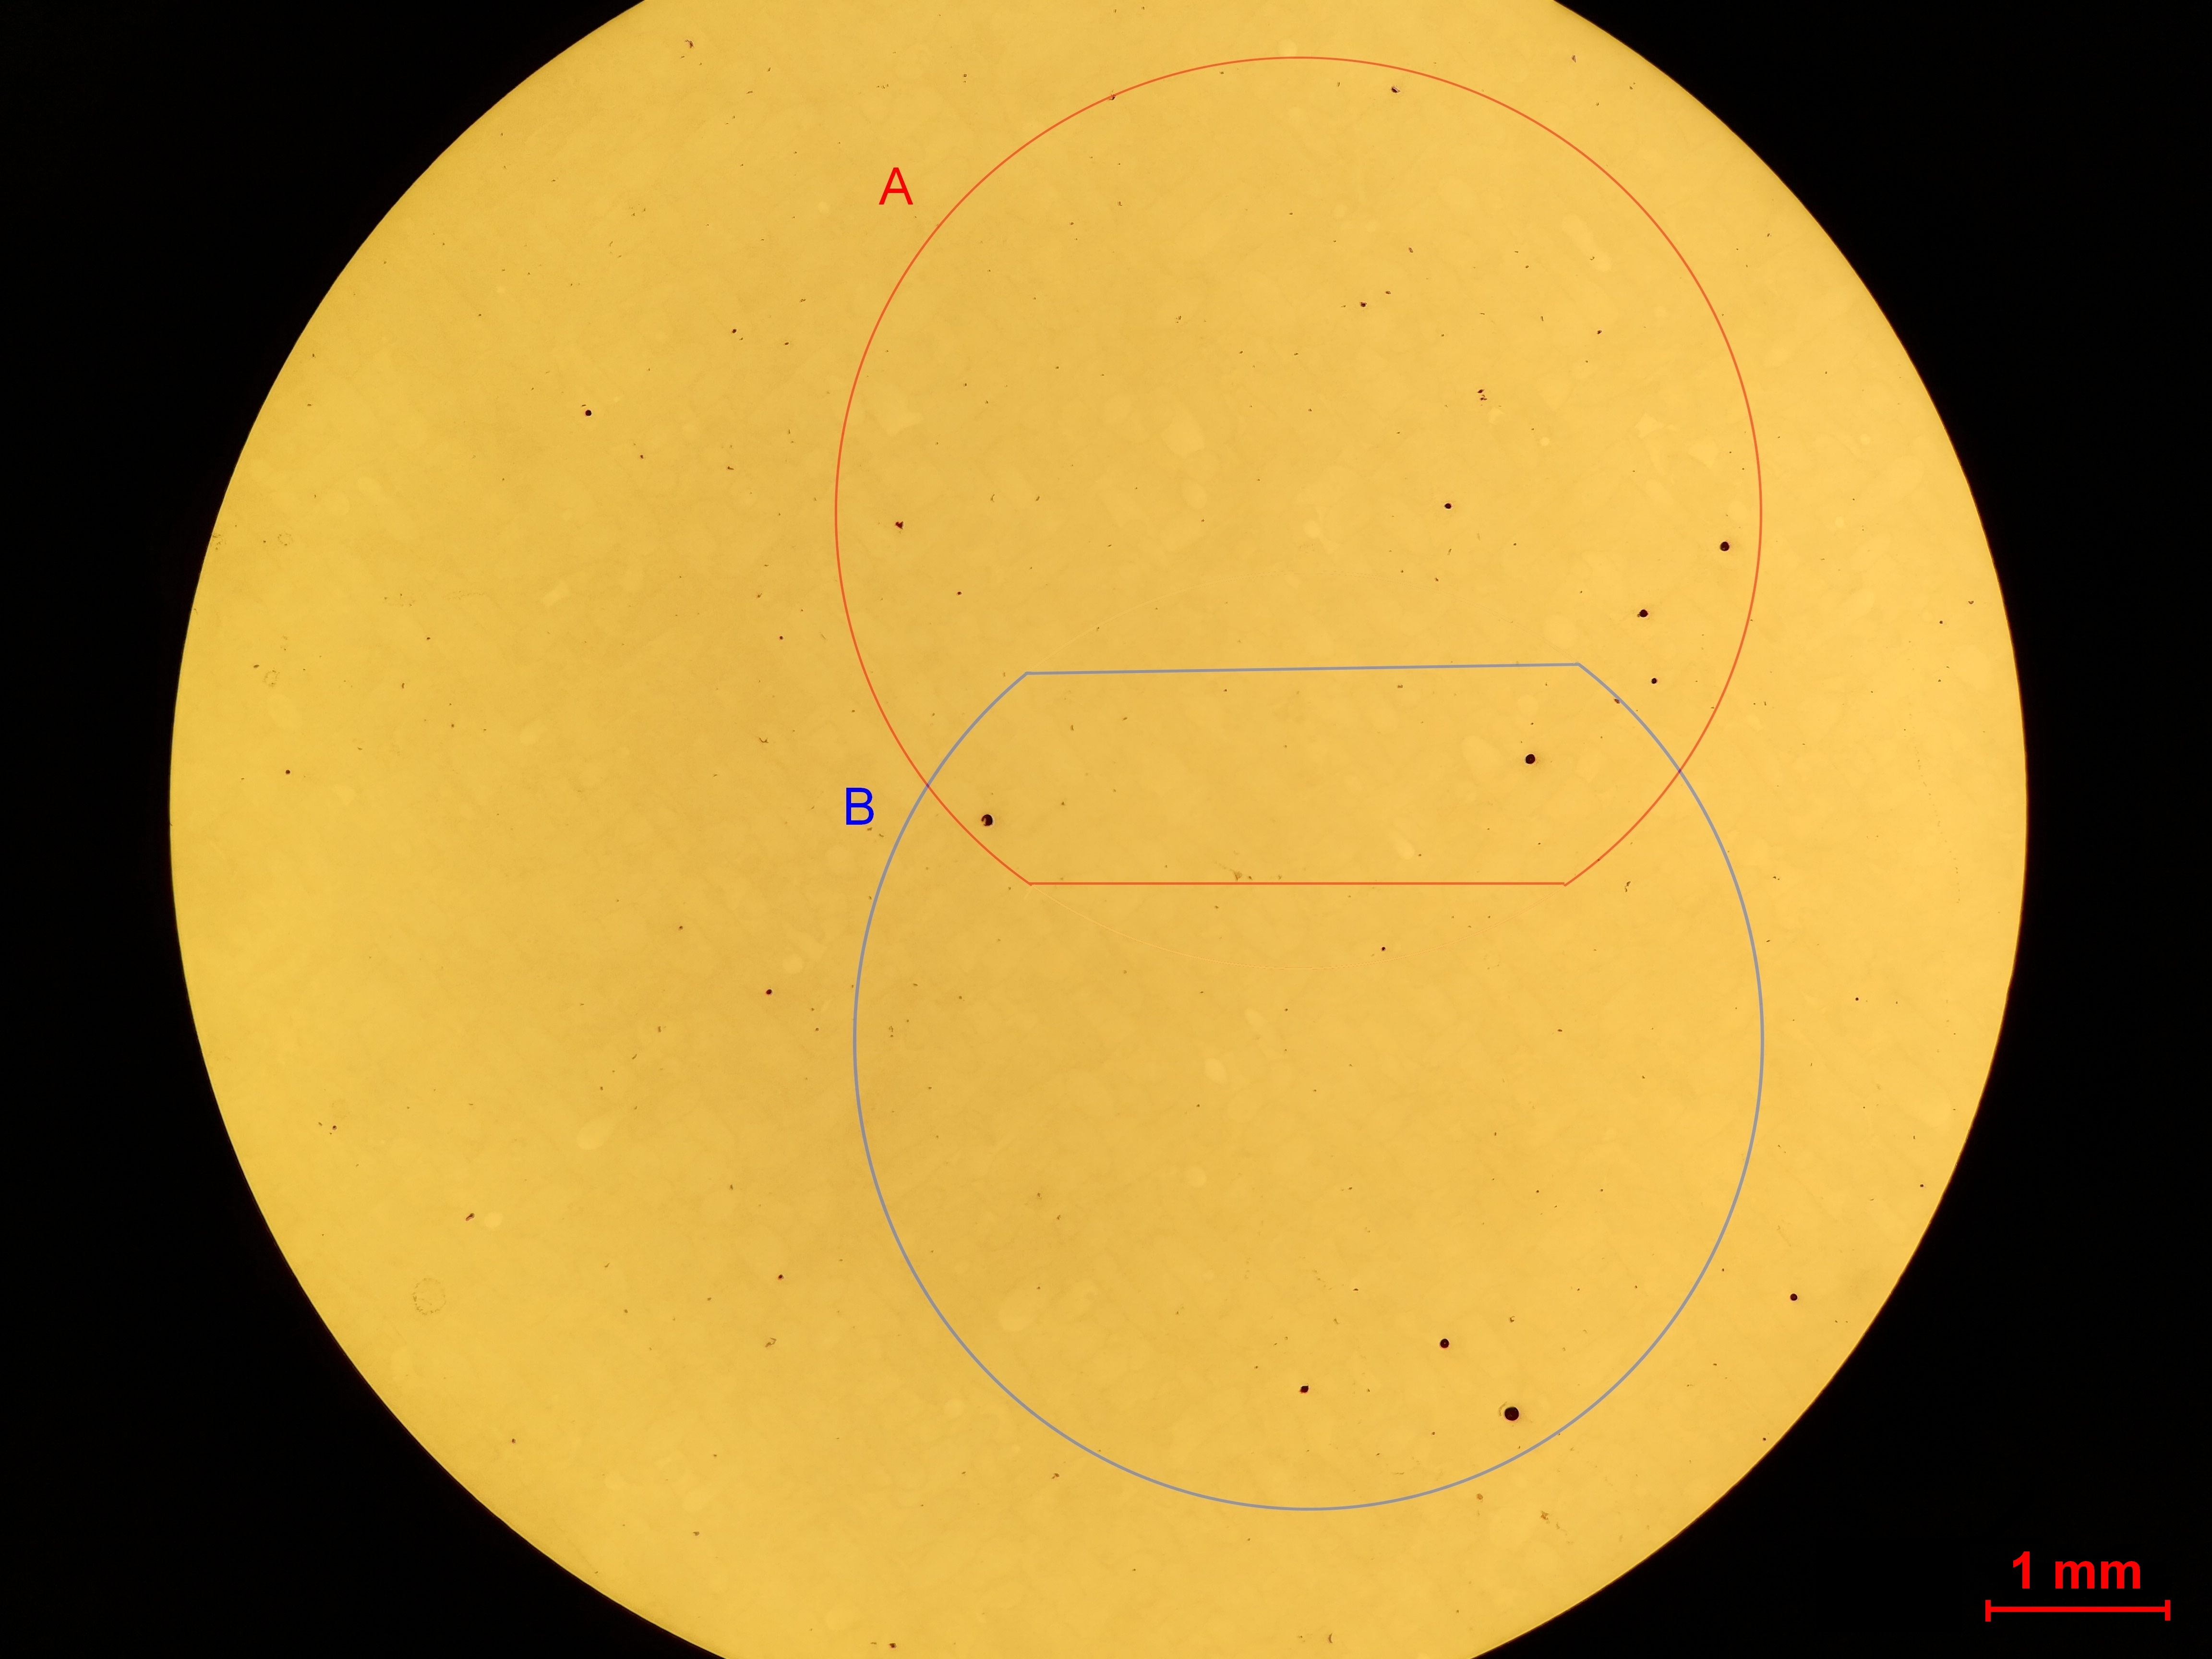
\includegraphics[scale=0.075]{Images/RODIA1}}
	\decoRule
	\caption[5x magnification picture of specimen X200-180319-cub1 and delimitation of the zones A and B]{5x magnification picture of specimen X200-180319-cub1 and delimitation of the zones A and B}
	\label{fig:RODIA1}
\end{figure}

\begin{figure}[ht]
	\centering
	\centerline{\includegraphics[scale=0.43]{Images/RODIAHist}}
	\decoRule
	\caption[Histograms of porosities areas occurrences from pictures of specimen X200-180319 on zone A under (a) 5x magnification (b) 10x magnification]{Histograms of porosities areas occurrences from pictures of specimen X200-180319 on zone A under (a) 5x magnification (b) 10x magnification. }
	\label{fig:RODIAH}
\end{figure}


The comparison of figures \ref{fig:RODIA2} (b) and (d) shows that much more small porosities are isolated if the resolution is refined. This is confirmed by the histograms on figure \ref{fig:RODIAH}. The threshold of porosity area for detection in the case of 5x magnification is 0.5625 [$\mu m^2$] whereas it is 0.14 [$\mu m^2$] for 10x magnification. This area corresponds to a pixel in each case. It is also worth noting that there is an overall tendency to overestimate the areas at lower resolution, which counterbalances slightly the low number of detected porosities. \\

\begin{figure}[ht]
	\centering
	\centerline{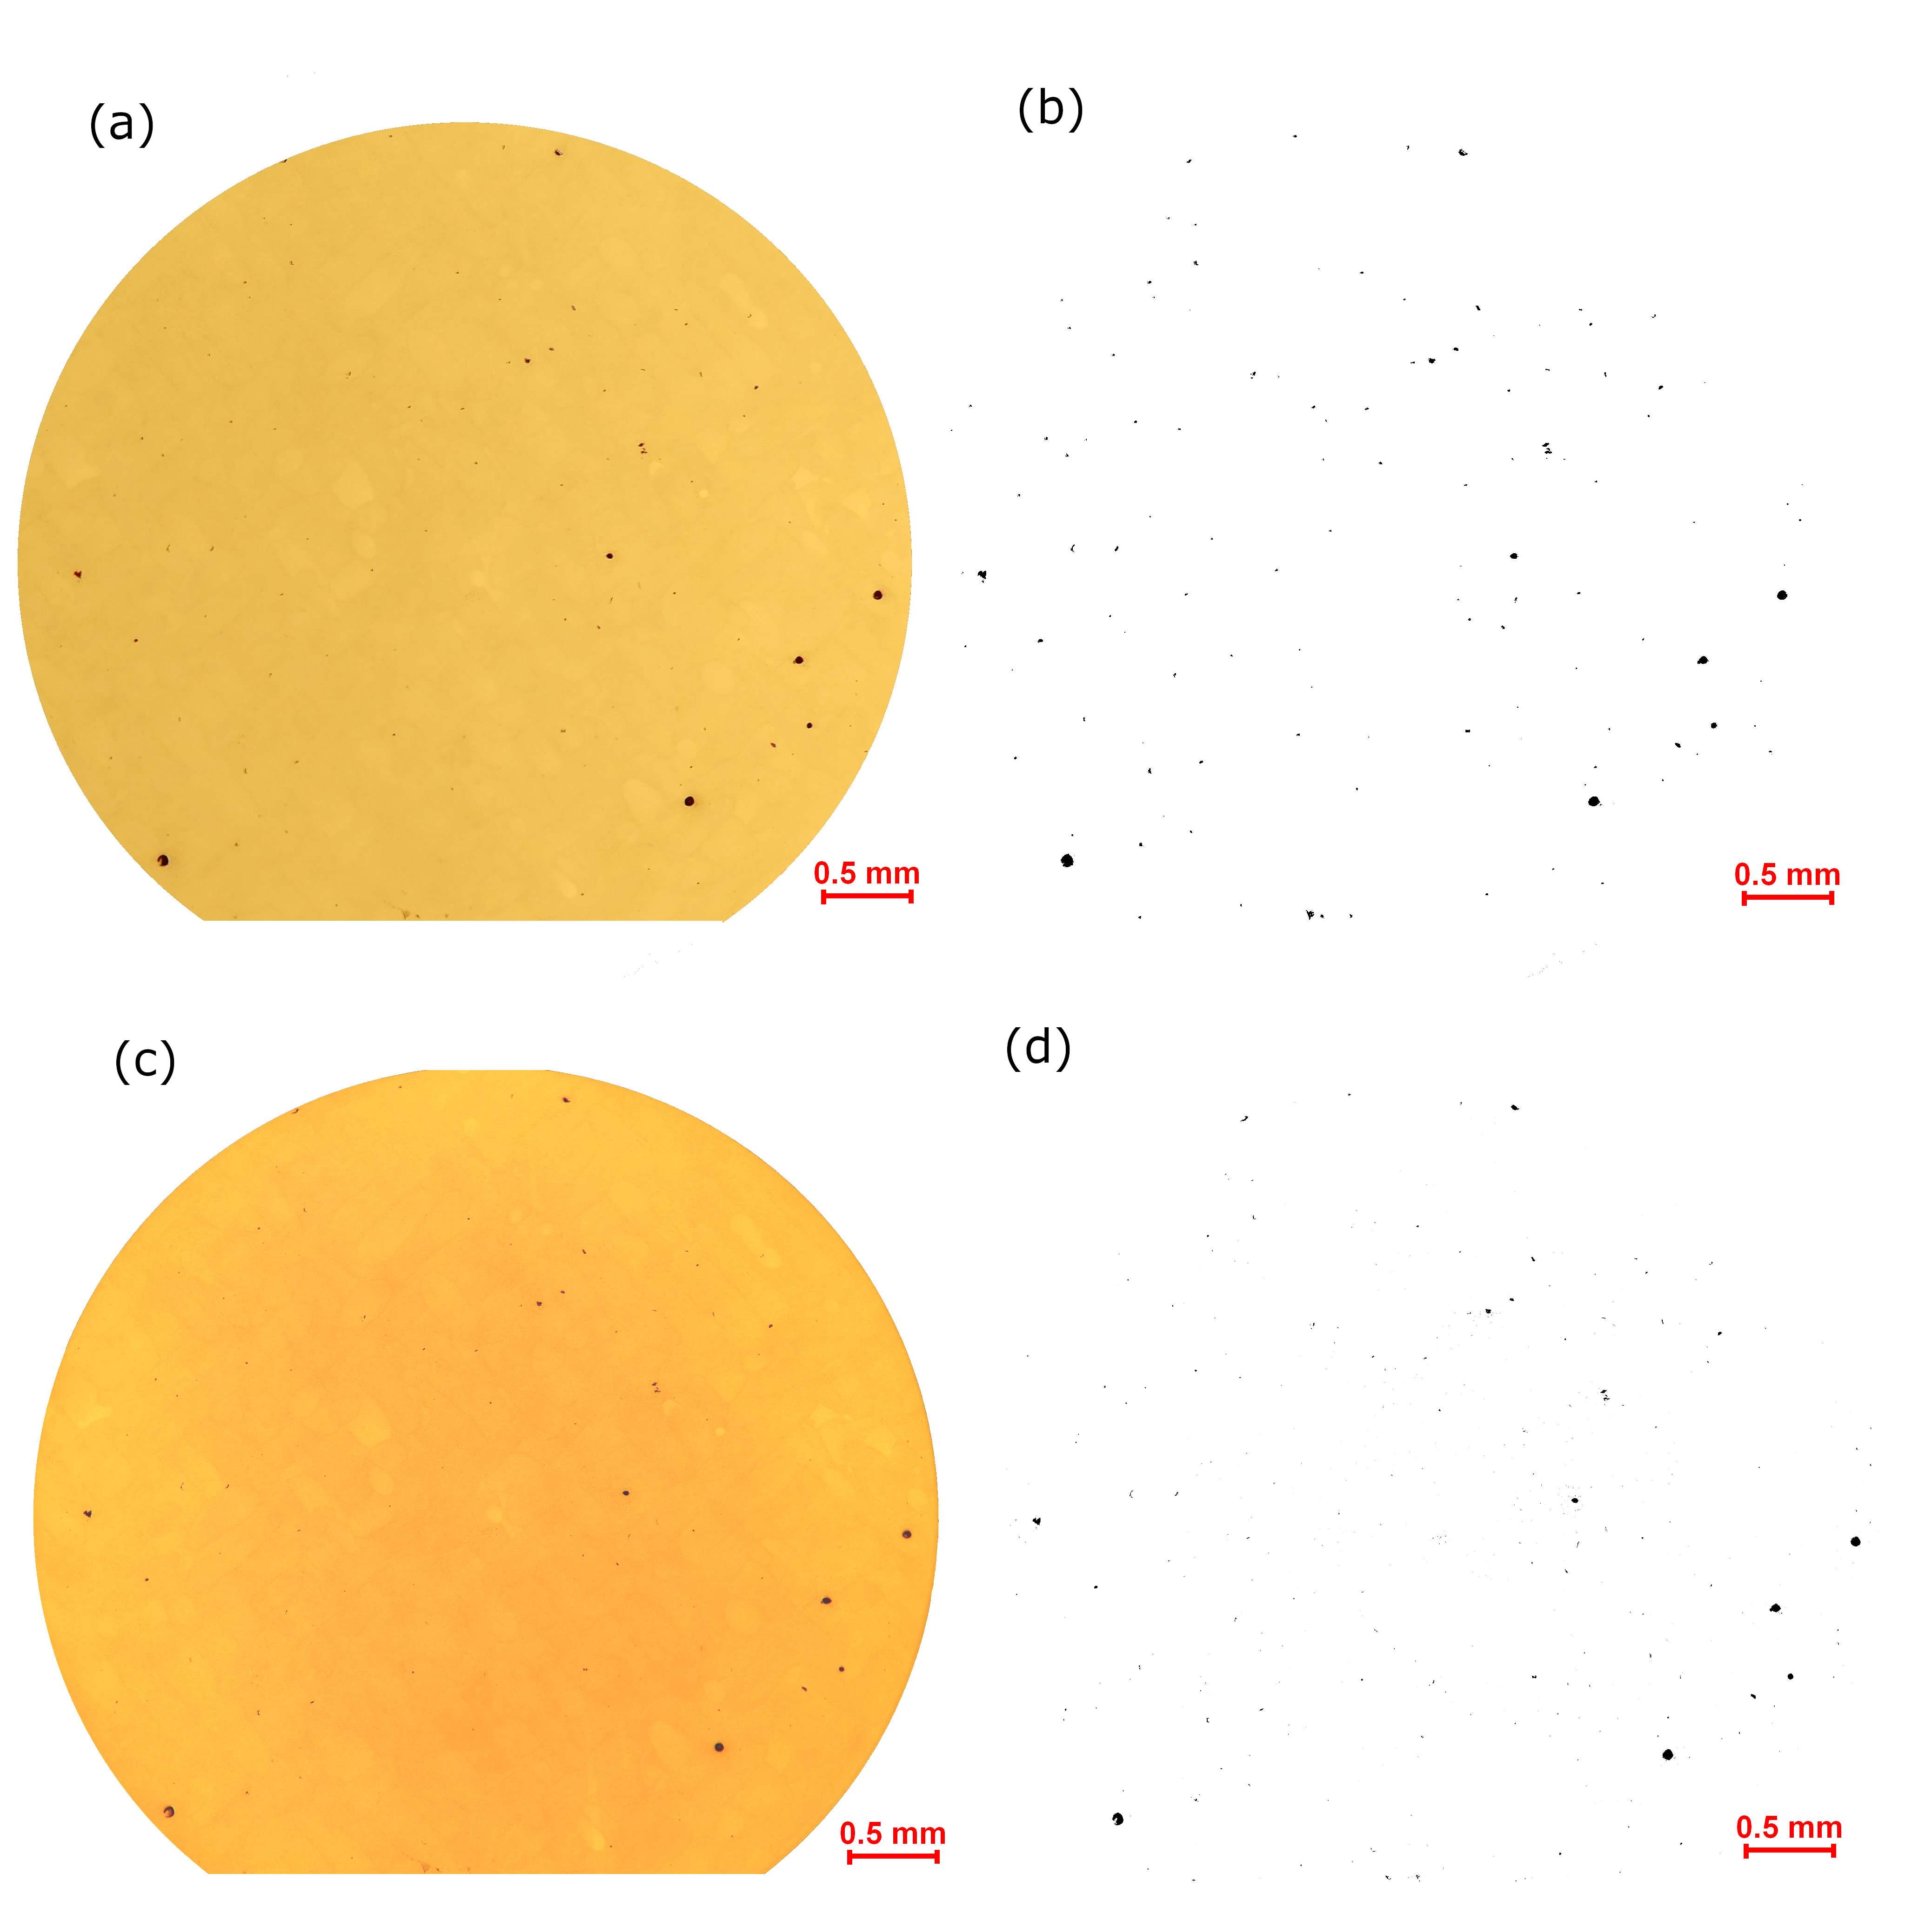
\includegraphics[scale=0.44]{Images/RODIA2}}
	\decoRule
	\caption[Zone A of specimen X200-180319-cub1: (a) Delimitation from original picture under 5x magnification (b) Porosities isolation from 5x magnification picture (c) Original picture under 10x magnification (d) Porosities isolation of 10x magnification picture]{Zone A of specimen X200-180319-cub1: (a) Delimitation from original picture under 5x magnification (b) Porosities isolation from 5x magnification picture (c) Original picture under 10x magnification (d) Porosities isolation of 10x magnification picture}
	\label{fig:RODIA2}
\end{figure}


The RODIA results for zones A and B are outlined in table \ref{tab:RODIASS}. It was observed that pictures with lower resolution have the tendency to lead to the overestimation of the relative density. The order of magnitude of the difference is of few hundredths of percent. The method is thus presumably positively biased. However, the observed effect is minor: this is probably due to the fact that the undetected porosities are the smallest, which influence the less the calculated density value.\\

\begin{center}
	\begin{table}[ht]
		\centerline{\begin{tabular}{|c|c|c|}
				\hline
				Zone & Magnification & Measured relative density [$\%$] \\
				\hline
				A & 5x  & 99.87\\
				A & 10x & 99.84\\
				B & 5x & 99.86\\
				B & 10x & 99.85\\
				\hline
		\end{tabular}}
		\caption[RODIA results for zones A and B of specimen X200-180317 with 5x and 10x magnification]{RODIA results for zones A and B of specimen X200-180317 with 5x and 10x magnification}
		\label{tab:RODIASS}
	\end{table}
\end{center}

Taking pictures at refined magnification could be considered to better the precision of the method. This would, however, require to augment the number of analysed pictures to have a sample of pictures as representative. A picture with doubled magnification covers indeed four times less surface. The number of analyses should thus be quadrupled to take as much information into account.\\

RODIA method required to make the assumption that the volumetric porosity fraction is equal the surface one. The dependability of this affirmation will now be discussed. Let us consider a cubic cell of side length D containing a spheric porosity of diameter D in its center (see figure \ref{fig:DDD}). The volumetric porosity fraction $f_v$ is:\\

$$f_v = \frac{\frac{\pi D^3}{6}}{D^3}= \frac{\pi}{6}$$

\begin{figure}[ht]
	\centering
	\centerline{\includegraphics[scale=0.64]{Images/DDD}}
	\decoRule
	\caption[Schematic of a spheric porosity of diameter D in a cubic cell of size length D]{Schematic of a spheric porosity of diameter D in a cubic cell of size length D}
	\label{fig:DDD}
\end{figure}

However, the surface porosity fraction depends on the observed pore diameter $D_{obs}$ which varies with the z coordinate of the surface plane crossing it: $\frac{D_{obs}(z)}{2}=\sqrt{(\frac{D}{2})^2-z^2}$. If we assume that there is a statistically significant number of pores of similar size, one can make the hypothesis that - in average - the observed diameter is the mean diameter $D_{mean}$:\\

$$ \frac{D_{mean}}{2}= \frac{\int_{-\frac{D}{2}}^\frac{D}{2} D_{obs}(z) dz}{D}=\frac{\pi D}{8}$$

This hypothesis is quiet coherent for small pores but not  for the largest: in most cases, a very small number of pores is significantly bigger than the others. If we still assume it to be true, the surface porosity fraction $f_s$ can be computed as follows:

$$f_s=\frac{\frac{\pi D_{mean}^2}{4}}{D^2}=\frac{\pi^3}{16 \cdot 4} \simeq 0.9253 f_v$$

It can thus be concluded that the method to measure the relative density is slightly intrinsically positively biased. The greater the porosity is, the bigger the bias. In the working range of $\rho_{rel}$ of this work, they can go from 0.01 to 0.03 [\%]. Combining this with the bias induced by the measures imperfections, one can conclude that RODIA should be used as a mean to estimate an upper limit for the relative densities.

\section{Density and hardness study}

\subsection{Parameters optimisation}

\subsection{Reproducibility}

\section{Characterisation of the as-built samples}

\subsection{Melt pools sizes and distribution}

\subsection{Microstructure}

\subsection{Residual stresses}

\subsection{Mechanical properties}
 [Critère de considère]
\section{Characterisation of the heat treated samples}

\subsection{Heating process}
Quand on chauffe à 300 deg, on chauffe déjà longtemps à plus de 200 deg

\subsection{Microstructure}

\subsection{Residual stresses}

While the usual stress-relief treatment for aluminium alloys -to hours holding at 300$^\circ$ C- does indeed relieve stresses inside the specimen, it also triggers significantly the diffusion of alloying elements, altering the material microstructure.

\subsection{Mechanical properties}


\subsection{Optimisation}



%\section{Mechanical testing}

\chapter{Conclusion}
\label{Chap6}
They incorporate in a synthetic way the main results and compare them with the
initial objectives. Generally, this final chapter also presents prospects for the continuation of the
work undertaken.
%\include{Chapitres/Chapitre1}
%----------------------------------------------------------------------------------------
%	THESIS CONTENT - APPENDICES
%----------------------------------------------------------------------------------------

\appendix % Cue to tell LaTeX that the following "chapters" are Appendices

% Include the appendices of the thesis as separate files from the Appendices folder
% Uncomment the lines as you write the Appendices

\include{Appendices/AppendiceA}
%% Appendix B

\chapter{Extract of Vickers hardness conversion table (HV10)} % Main appendix title

\label{AppendixB} % For referencing this appendix elsewhere, use \ref{AppendixA}

\begin{center}
\begin{table}[ht]
\noindent\makebox[\textwidth]{\begin{tabular}{|c|c |c |c| c|c|c|c|c|c|c|}
    \hline
    Diagonal length [mm] & 0 &1&2&3&4&5&6&7&8&9\\
\hline 
\hline   
    0.34 & 160 &160&159&158&157&156&155&154&153&152\\
    0.35&151.4&150.5&149.7&148.8&148.0&147.1&146.3&145.5&144.7&143.9\\ 
    0.36&143.1&142.3&141.5&140.7&140.0&139.2&138.4&137.7&136.9&136.2\\
    0.37&135.5&134.7&134.0&133.3&132.6&131.9&131.2&130.5&129.8&129.1\\
    0.38&128.4&127.7&127.1&126.4&125.8&125.1&124.5&123.8&123.2&122.6\\
    0.39&121.9&121.3&120.7&120.1&119.5&118.9&118.3&117.7&117.1&116.5\\
    0.40&115.9&115.3&114.8&114.2&113.6&113.1&112.5&111.9&111.4&110.9\\
    0.41&110.3&109.8&109.3&108.7&108.2&107.7&107.2&106.6&106.1&105.6\\
    0.42&105.1&104.6&104.1&103.6&103.1&102.7&102.2&101.7&101.2&100.8\\
    0.43&100.3&99.8&99.4&98.9&98.5&98.0&97.6&97.1&96.7&96.2\\
    0.44&95.8&95.3&94.9&94.5&94.1&93.6&93.2&92.8&92.4&92.0\\
    0.45&91.6&91.2&90.8&90.4&90.0&89.6&89.2&88.8&88.4&88.0\\
    0.46&87.6&87.3&86.9&86.5&86.1&85.8&85.4&85.0&84.7&85.3\\
    0.47&84.0&83.6&83.2&82.9&82.5&82.2&81.8&81.5&81.2&80.8\\
    0.48&80.5&80.2&79.8&79.5&79.2&78.8&78.5&78.2&77.9&77.6\\
    0.49&77.2&76.9&76.6&76.3&76.0&75.7&75.4&75.1&74.8&74.5\\
    0.50&74.2&73.9&73.6&73.3&73.0&72.7&72.4&72.1&71.9&71.6\\
    0.51&71.3&71.0&70.7&70.5&70.2&69.9&69.6&69.4&69.1&68.8\\
    0.52&68.6&68.3&68.1&67.8&68.5&67.3&67.0&66.8&66.5&66.3\\
    0.53&66.0&65.8&65.5&65.3&65.0&64.8&64.5&64.3&64.1&63.8\\
    0.54&63.6&63.4&63.1&62.9&62.7&62.4&62.2&62.0&61.7&61.5\\    \hline
\end{tabular}}

\caption[Extract of Vickers hardness conversion table (HV10)]{Extract of Vickers hardness conversion table (HV10)}
\label{tab:compo}
\end{table}
 \end{center}

%% Appendix B

\chapter{Procedure for the confidence intervals computation} % Main appendix title

\label{AppendixC} % For referencing this appendix elsewhere, use \ref{AppendixA}

\section{Apparent relative density}

The hydrostatic weighting method requires to weight the analysed samples two times; once in air and once in water. The measurements data of the two weightings are subjected to a certain spreading - especially large in the case of underwater measurements. Both of the tests imprecisions must thus be taken into account when computing the confidence intervals (CI) for $\rho_{a,rel}$. The following procedure was followed:

\begin{itemize}
\item Computation of the standard deviation $SD_x$ for the two data samples of observed mass values \{$x_1$,$x_2$,...$x_N$\} with the formula below:

$$SD_x=\sqrt{\frac{\Sigma^N_{i=1}(x_i-\bar{x})^2}{N-1}} $$

where is N the sample size and $\bar{x}$ is the mean of the observed values.

\item Determination of the CI range at a 95 [\%] confidence level for each data sample with the following formula:

$$CI= \bar{x} \pm 1.96 \frac{SD_x}{\sqrt{N}}$$

\item Use of the mean values incremented by the extreme values of the CI for both $W_a$ and $W_w$ in the formula:


$$\rho_a=\frac{W_a}{W_a-W_w} \cdot \rho_w $$

so as to maximise the absolute value of the difference with $\bar{x}$. This difference is then equal to the CI half length for a 95 [\%] confidence level. One should note that the following hypotheses were made: the method is unbiased and the tests are depending one on another. The latter hypothesis maximises the CI. It is used for reasons of caution. The validity of the hypotheses is discussed in section \ref{DDMA}.
\end{itemize}

\section{Vickers hardness}

Hardness measurements of a given sample are also prone to having a certain variability. CI must thus be computed to assess the method precision. The CI is first calculated for the data sample composed of the mean diagonals length of the indents. For this purpose, one follows the same two first steps as for the hydrostatic weighting. The CI range is then multiplied by 800 to find the hardness's one. This is done in accordance with the observation that the maximal hardness variation for a change of 0.001 [mm] is 0.8 [HV] in table \ref{tab:HV} for $H_v<147.1 $[HV].% This is the origin of the factor 800. 

%----------------------------------------------------------------------------------------
%	BIBLIOGRAPHY
%----------------------------------------------------------------------------------------

\printbibliography[heading=bibintoc]

%----------------------------------------------------------------------------------------

\end{document}  
